\chapter{Grundlagen}

\section{Was ist \textit{The Learning Triangle} (TLT)}

Dieser Abschnitt befasst sich mit der Vorlage für dieses Projekt, The Learning Triangle. Es werden das grundlegende Prinzip sowie die wichtigsten Regeln erklärt und auch die technische Seite wird erläutert. Abschließend wird beschrieben, wie TLT im Zuge dieser Arbeit weiterverwendet wird. 

\subsection{Grundidee}

Im Rahmen des Software Engineering Kurses an der DHBW Karlsruhe sollte in Gruppen von zwei bis vier Studenten ein eigens gewähltes Projektthema erarbeitet werden. Eines der Projekte aus dem Studienjahr 2016/17 war TLT. Die Grundidee des Projektes war die Simulation des Verhaltens von Kreaturen, den namensgebenden \grqq Triangles\glqq{}. Sie sollten sich bewegen und auf ihre Umwelt reagieren, mit dem Ziel, solange wie möglich zu überleben. Das dafür nötige Wissen wurde ihnen jedoch nicht mithilfe einprogrammierter Regeln vorgegeben, sie sollten es eigenständig aufbauen. Am Allerbesten eignet sich dafür künstliche Intelligenz. 

\subsection{Regelwerk}

Zu Beginn musste ein Rahmen festgelegt werden, der die Regeln des Programms beschreibt. Dabei wird zwischen verschiedenen Regelbereichen unterschieden, den Regeln für die Triangles, den Regeln für die Oberwelt und den allgemeinen Spielregeln. Auf alle soll im Folgenden eingegangen werden.

\subsubsection{Allgemeine Regeln}

Die Allgemeinen Regeln beschreiben die Zusammenhänge der einzelnen Spielelemente. Pro Spiel existiert eine Oberwelt auf der sich eine beliebige Menge an Triangles befindet. Gesteuert werden diese Triangles nicht durch vorhandene Algorithmen, die wissen welcher Pfad der Beste ist, sondern durch eine künstliche Intelligenz, die sich dieses Wissen erst erarbeiten muss. 

Das Spiel startet mit der Erstellung einer Oberwelt, gefolgt vom eigentlichen Spielablauf mit dem Abschließen des Spiels durch den Tod aller Triangles. Ein Siegkriterium ist nicht vorhanden. Wie die Oberwelt erstellt wird kann in \ref{subsubsec_oberweltregeln} nachgelesen werden. Der Spielablauf an sich erfolgt in kurzen Zyklen. In jedem Zyklus bewegt sich jedes Triangle ein Feld in eine von der KI bestimmten Richtung. Die Feldaktionen werden ausgeführt und ein neuer Zyklus beginnt.

Das durch die allgemeinen Regeln festgelegte Ziel ist eine möglichst lange Lebenserhaltung aller Triangles. Da ein Algorithmus mit dieser Aussage wenig anfangen kann und es zu ungewollten Lösungen kommen kann, muss das Ziel greifbarer ausgedrückt werden. Deshalb lautet das der AI mitgeteilte Ziel, so viel Strecke wie möglich zurückzulegen, was sich nur durch eine lange Lebensspanne aller Triangles realisieren lässt. Bereits in der Vergangenheit gegangene Wege erhöhen den Distanzwert erneut, sodass es keinen Maximalwert gibt.

\subsubsection{Oberwelt-Regeln}
\label{subsubsec_oberweltregeln}
Diese Regeln beschreiben, wie die Oberwelt erstellt wird und welche Vorgaben dabei beachtet werden müssen. Die wichtigste Eigenschaft der Map ist die beliebig große quadratische Oberwelt, bestehend aus einzelnen, ebenfalls quadratischen Feldern. Diese Felder besitzen verschiedene Eigenschaften welche in Tabelle \ref{tbl_fields} näher erläutert werden. \\

\begin{center}
\label{tbl_fields}
\begin{tabular}{ | p{1.5cm} |p{3cm} | p{8.5cm}| c r r }
\hline
Bild & Feld-Typ & Eigenschaft \\
\hline

\includegraphics[scale=0.6]{bilder/Style-Classic_Normal_Field.png} & Normal-Field & Das Standard-Feld, welches keine Effekte auf das Triangle wirken lässt. Es kann betreten und verlassen werden. \\ 
\hline

\includegraphics[scale=0.6]{bilder/Style-Classic_Wall_Field.png} & Wall-Field & Auf der Oberwelt gibt es nicht passierbare Felder, die das Triangle nicht überqueren kann. Diese Felder sind Wall-Fields. \\ 
\hline

\includegraphics[scale=0.6]{bilder/Style-Classic_Energy_Field.png} & Energy-Field & Das Triangle besitzt eine begrenzte Menge Energie. Diese wird um eine festgelegte Menge erhöht, sollte dieses Feld betreten werden. Dieser Vorgang ist einmalig, das Energiefeld verliert seine Eigenschaften bei Kontakt. Dies verhindert, das die AI Triangles einfach zwischen Energie-Feldern und anderen Feldern hin- und herbewegt, da sie ohne diese Regel dafür unbegrenzt Energie und Strecke erhalten würde.\\
\hline

\includegraphics[scale=0.6]{bilder/Style-Classic_Poison_Field.png} & Poison-Field & Bei jedem Schritt braucht ein Triangle Energie. Das berühren dieses Feldes erhöht die nötige Menge Energie einer Triangle-Bewegung für einige zukünftige Zyklen des Spielablaufs. \\ 
\hline

\includegraphics[scale=0.6]{bilder/Style-Classic_Death_Field.png} & Death-Field & Bei Kontakt mit diesem Feld verliert das Triangle seine ganze Energie und stirbt. \\ 
\hline
\end{tabular}
\end{center}

Die Oberwelt kann über zwei verschiedene Arten erstellt werden. Es ist möglich, eine vorhandene, korrekt formatierte Datei einzulesen und als Map zu verwenden, die Oberwelt kann aber auch zufällig generiert werden. Dabei lässt sich einstellen, wie hoch die Wahrscheinlichkeit für die einzelnen Felder sein soll. Jede generierte Oberwelt lässt sich für die zukünftige Verwendung wieder in eine Datei speichern. Mithilfe der Implementierung eines Mapbuilders lassen sich diese Dateien bearbeiten.

\begin{figure}
\centering
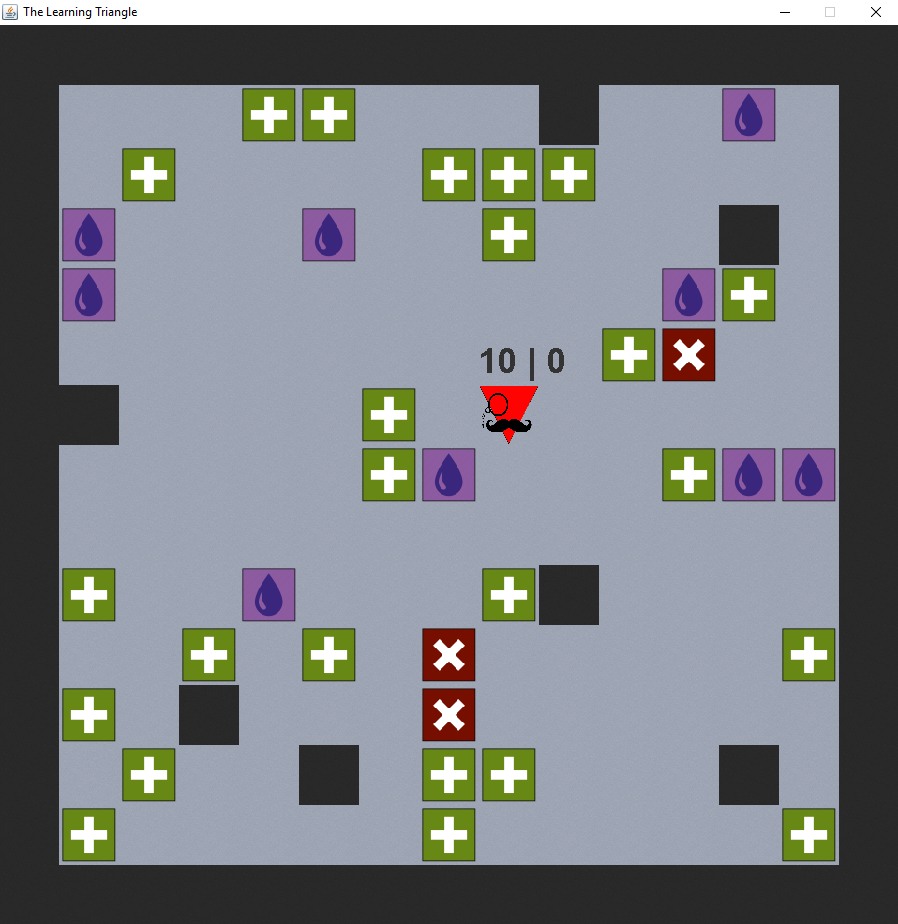
\includegraphics[scale=0.5]{bilder/TLT_Game.PNG}
\caption{Beispiel für eine zufällig erstellte Oberwelt}
\label{BeispielMapTLT}
\end{figure}


\subsubsection{Triangle-Regeln}

Für jede Instanz eines Triangle gelten Regeln. Diese beschreiben unter anderem auch die Fähigkeiten eines Triangles. Grundlegend gesehen ist die Implementierung eines Triangles eine sehr vereinfachte Variante eines kleinen Lebewesens. Es besitzt eine festgelegte Menge an Energie, welche es bei Bewegung verbraucht. Ist alle Energie verbraucht, stirbt das Triangle. Das Ziel von TLT war es, solange wie möglich zu überleben. Zu diesem Zweck muss das Triangle ausreichend oft Energie-Felder betreten. Um diese zu finden besitzt jedes Triangle ein Sichtfeld, bestehend aus allen Felder um die aktuelle Position herum verteilt. Der Radius ist dabei festgelegt. Die Bewegung des Triangles erfolgt in vier mögliche Richtungen: Norden, Süden, Osten und Westen. Die Entscheidung in welche Richtung gegangen werden soll trifft das Triangle nicht selbst. Diese Aufgabe wird von dem implementierten AI-Algorithmus getroffen.

\subsection{Bisherige Technische Seite des Projektes TLT}
\label{bisherigeTechnikTLT}

Technisch basiert TLT auf Java. Es existieren drei verschiedene Schichten im bisherigen Projekt: Die Anwendungsoberfläche, in der nachvollzogen werden kann was gelernt wurde und was dann mit den Triangles passiert, wird dieses Wissen angewendet. Darunter liegt das Regelwerk, welches die beschriebenen Regeln implementiert und gewährleistet, dass keine unerwarteten Dinge passieren. Hier werden auch alle Parameter konfiguriert. Den Abschluss bildet die Implementierung des \textit{Deep Learning} Algorithmus, im bisherigen Projekt war das die Bibliothek DeepLearning4Java. Dabei wurde ein neuronales Netzwerk aufgebaut welches als Eingabe das Sichtfeld eines Triangles erhält und als Ausgabe eine Richtung vorhersagt. Verwendet wurde dafür \textit{Reinforcement Learning} (siehe Kapitel \ref{machinelearning_ansaetze}), der Algorithmus wurde also fortlaufend mit einer Fitness bewertet. Perfekt ausgereift war die Implementierung der AI noch nicht, an vielen Stellen hätte noch gearbeitet werden können.

\subsection{Weiterverwendung des Projektes TLT}

Im Zuge dieses Projektes soll TLT zu einem \textit{Educational Game} werden. Verschiedene Begriffe und Algorithmen sollen erklärt werden. Damit das gut funktioniert ist eine häufige Neuimplementation vieler bereits entwickelter Bestandteile in leicht abgeänderter Form nötig. Das dieser Prozess möglichst wenig Aufwand verursacht und gut funktioniert muss eine klare Trennung zwischen den einzelnen technischen Bereichen geschaffen werden. TLT muss möglichst modular und austauschbar sein. Die bisher vorhandene Struktur ist für dieses Ziel von großem Nutzen, auch in Zukunft sollen die drei Schichten beibehalten werden. Ergänzt wird TLT durch eine weitere wichtige Schicht, in der die Daten gespeichert werden. Damit sind vor allem Erklärungstexte und Spielparameter gemeint.

Die Flexibilität der Regeln und Parameter ist eine große Stärke von TLT. Dies ermöglicht die fast uneingeschränkte Weiterverwendung des Projektes im Zuge der Erstellung eines \textit{Educational Game}. So werden einige der im Kommenden beschriebenen Regeln für spezifische Aufgaben angepasst oder aufgehoben, wieder andere werden dafür ins Regelwerk aufgenommen. Die Grundstruktur bleibt dabei bestehen.

\section{Was ist ein Educational Game}

\subsection{Definition}

\textit{Educational Game}, Lernspiel oder didaktisches Spiel wie die Spielwissenschaft solche Spiele bezeichnet, es gibt viele Begriffe, die jedoch ein und das selbe bezeichnen. \\

\begin{addmargin}[25pt]{0pt} 
\glqq An \textit{Educational Game} is a game designed to teach humans about a specific subject and to teach them a skill.\grqq \cite{F_DefinitionEducationalGame_3.2}
\end{addmargin}

\ \\ Ein \textit{Educational Game} ist demnach ein Spiel, das dazu gedacht ist, Menschen über ein bestimmtes Thema aufzuklären und ihnen eine Fertigkeit beizubringen. Das Ziel ist es, das Wissen auf eine Art und Weise zu vermitteln welche Spaß macht. Dabei ist die Form des \textit{Educational Game} völlig frei wählbar. Es kann sowohl als Brettspiel vorliegen, als auch ein Kartenspiel oder Computerspiel sein. 

Allerdings ist eine genaue Abgrenzung zwischen einem normalen Spiel und einem \textit{Educational Game} oftmals nicht einfach. Denn auch ein normales Spiel vermittelt auf irgendeine Art und Weise Wissen und Fertigkeiten. Diese Art von lernen wird auch \glqq Inzidentelles Lernen\grqq{} genannt. \glqq Beim inzidentellen Lernen handelt es sich um einen Vorgang, bei dem Informationen nebenbei (unabsichtlich) aufgenommen werden. Das bedeutet, wir lernen viele Inhalte, ohne dass eine Lernabsicht vorliegt. Der Anteil der unabsichtlichen Lernprozesse ist mindestens so groß wie der Anteil jener Lernprozesse, bei denen es eine Lernabsicht gibt. \grqq ~\cite{F_InzidentellesLernen_3.2} 

\subsection{Elemente eines Educational Game}
Die große Frage ist: Was machen \textit{Educational Games} anders? Dafür ist es hilfreich einen Blick in deren Vergangenheit zu werfen. Zunächst gab es einfache Vokabeltrainer, die über ein Belohnungssystem den Lernenden motivierten. Eine richtige Eingabe gab Punkte, falsche Angaben wurden über Punktabzug bestraft. Die nächste Stufe stellten interaktive Enzyklopädien dar. Der Spieler konnte darin seine Umgebung wie eine Art Museum erkunden und so die Lerninhalte selbständig erarbeiten. Inzwischen werden durch \textit{Educational Games} Mikrowelten generiert, in denen der Lernstoff spielerisch präsentiert wird. Meist wird dabei eine interaktive Geschichte erzählt. 

Wo liegen nun also die Unterschiede zum normalen Frontal-Unterricht? Als erstes sei das Belohnungssystem zu erwähnen. Das gibt es in der Form an Schulen oder Universitäten nicht. Dort wird eher ein Fehlerbestrafungssystem praktiziert. Das heißt, der Schüler lernt oftmals bloß aus Angst vor den Konsequenzen den Stoff. In der Psychologie wird diese Art von Motivation auch extrinsisch genannt. Das Problem dieser Form von Motivation ist, dass sie nur bestehen bleibt, solange die Leistung auch überprüft wird. \textit{Educational Games} hingegen setzen auf die intrinsische Motivation. Sie kommt im Gegensatz zur extrinsischen Motivation nicht von außen, sondern aus dem Innern. Das heißt die Aufgaben, welche erledigt werden müssen entsprechen den eigenen Wünschen. Vereinfacht gesagt wird das Spielen des \textit{Educational Games} zum eigenen Wunsch des Spielenden, da durch das Belohnungssystem ein Anreiz geschaffen wird, weiter zu spielen und somit auch zu lernen. Ein weiterer Vorteil den \textit{Educational Games} bieten, liegt im \glqq Trial-and-Error \grqq Prinzip. Der Spielende kann Dinge ausprobieren und aus den Fehlern lernen. Da Fehler an Schulen oftmals mit negativen Gefühlen und Konsequenzen verbunden werden, fällt der Effekt des Sprichworts \glqq aus Fehlern lernen \grqq oftmals weg. Der Vorteil den hier \textit{Educational Games} mitbringen liegt darin, dass durch das Fehlen von Erwartungen an einen direkten Nutzen, Fehler nicht negativ ins Gewicht fallen \cite{F_VorteileEducationalGames_3.2.2}

Was braucht es, damit ein \textit{Educational Game} erfolgreich ist? Zunächst sollte das Spielen Spaß machen und zum weiterspielen anregen. Dies kann zum Beispiel in Form einer interaktiven Geschichte erreicht werden. Ein positiver Nebeneffekt einer Geschichte ist, dass der Lernaktivität ein Sinn gegeben wird. Jedoch muss darauf geachtet werden, dass das Spielziel dem Lernziel entsprechen sollte. Das heißt, um ein Level weiter zu kommen, muss der vermittelte Lerninhalt verstanden sein. Ein weiterer Bestandteil, welcher ein \textit{Educational Game} erfolgreich machen kann ist die Möglichkeit der sozialen Interaktion. Das kann zum Beispiel dadurch erreicht werden, dass Klassenkameraden zusammen wirken müssen, um eine Aufgabe zu lösen, oder in einem anderen Spielmodi gegeneinander antreten können, um eine Rangliste untereinander auszuspielen. \cite{ F_erfolgreicheEducationalGames_3.2}

\subsection{Beispiele}
In \textit{Educational Games} wird in erster Linie Wissen vermittelt.Die Tabelle \ref{tbl_educationalGames} enthält einige Beispiele und was das jeweilige \textit{Educational Game} vermitteln möchte.\newline

\begin{center}
\label{tbl_educationalGames}
\begin{tabular}{ |p{3cm} | p{10cm}| c r }
\hline
Spiel & Lerninhalte \\
\hline
Boggle, Galgenmännchen & Um zu gewinnen muss jeweils ein deutsches Wort beziehungsweise so viele deutsche Wörter wie möglich gefunden werden. Dabei kann die Rechtschreibung geübt und der Wortschatz erweitert werden. Diese Spiele eignen sich auch dafür, Fremdsprachen zu lernen. \\  
\hline
Stadt-Land-Fluss & In diesem Spiel können die geografischen Kenntnisse der Spieler erweitert werden. \\
\hline
Schiffe versenken & Durch Schiffe versenken lernt der Spieler den Umgang mit Koordinatensystemen.   \\ 
\hline
Brain It On! & In diesem Smartphone Spiel müssen verschiedene Rätsel durch zeichnen von Formen gelöst werden. Dabei muss der Spieler die Gesetze der Physik, wie zum Beispiel die Schwerkraft beachten um das jeweilige Ziel zu erreichen. \\ 
\hline
\end{tabular} 
\end{center} 

Unter den Begriff \textit{Educational Game} fallen auch Spiele, welche die sozialen Fertigkeiten des Spielenden erhöhen. Eine Kombination aus der Vermittlung von Wissen und sozialen Kompetenzen gibt es natürlich auch. Ein Beispiel hierfür ist das Waldschattenspiel. In diesem Brettspiel müssen die Spieler gemeinsam gegen das Licht in Form eines Teelichts spielen. Das Spiel wird im Dunklen gespielt, damit der Unterschied zwischen Licht und Schatten besser zu erkennen ist. Auf dem Spielbrett gibt es verschiedene Wege und einige verteilte 3D Tannenbäume hinter denen sich Spielfiguren vor dem Licht verbergen können. Ziel des Spiels ist ein gemeinsames Treffen im Schatten eines Tannenbaumes. Gerät eine Spielfigur ins Licht müssen die Mitspieler versuchen, durch Bewegen des Lichts, die Figur wieder zu befreien. Das Waldschattenspiel vermittelt also nicht nur den Wissenschaftlichen Aspekt von Licht und Schatten sondern fördert die Kooperation mit anderen. \cite{F_Lernspiel_3.2}

\section{Was ist AI}

In diesem Abschnitt werden die wichtigsten Begriffe rund um \textit{Artificial Intelligence} erklärt. Dabei ist jedoch eine grundlegende wichtige Annahme wichtig. Durch den neuen Aufschwung von Machine Learning werden viele bereits seit vielen Jahren existierende Methodiken und Begriffe von vielen Seiten neu betrachtet und es gibt deshalb keine klare Definition für jeden einzelnen Fachbegriff. Stattdessen gibt es Meinung, wie genau Begriffe zu definieren sind, die aber immer wieder validiert und/oder angepasst werden. Das erschwert die Situation, klare Aussagen zu treffen. Die nachfolgenden Erklärungen sind deshalb unter Anbetracht des aktuellen Datums und der Freiheit, auch anders definiert sein zu können zu lesen. Beruhigend ist, das keine großen Unterschiede zwischen den Auslegungen existieren, sondern nur kleine Differenzen. Keine der Definitionen ist deswegen grundlegend falsch oder anders.

\subsection{Definitionen} 

Zunächst soll der Begriff AI genauer definiert werden. \\

\begin{addmargin}[25pt]{0pt} 
\glqq Artificial intelligence (AI) is an area of computer science that emphasizes the creation of intelligent machines that work and react like humans. Some of the activities computers with artificial intelligence are designed for include: Speech recognition, Learning, Planning, Problem solving\grqq \cite{F_AIDfinition_3.3.1}
\end{addmargin}

\ \\ AI ist ein Bereich der Informatik, in dem an künstlichen Intelligenzen geforscht wird. Allerdings ist das Forschungsgebiet keinesfalls geschlossen. Viele andere Wissenschaften wirken bei der Entwicklung mit. Es geht darum, Systeme zu entwickeln, die Aufgaben erledigen können, bei denen normalerweise menschliches Denken benötigt wird. Dazu gehören zum Beispiel Spracherkennung, Bilderkennung, Übersetzungen, Entscheidungen anhand mehrerer Faktoren richtig treffen und neue Dinge zu lernen. Entgegen der weit verbreiteten Vorstellungen muss eine AI nicht unbedingt die Fähigkeit haben, dazuzulernen. Viele Systeme klassifizieren \glqq nur\grqq{} die vorliegenden Daten, oder extrahieren Wissen daraus. Ein ebenfalls weit verbreiteter Irrtum ist, dass eine AI intelligent ist, jedoch wird mittels Mathematik und Informatik lediglich intelligentes Verhalten simuliert. Von der Schaffung eines Bewusstseins ist die Forschung noch unabsehbar weit entfernt.

\paragraph{Starke künstliche Intelligenz} Die Schaffung eines Bewusstseins wird durch den Begriff starke künstliche Intelligenz beschrieben. Sie beschäftigt sich damit, menschliches Denken zu mechanisieren, damit eine Maschine wie ein Mensch reagieren kann. Wie oben schon beschrieben, ist dieser Bereich von AI eher eine Vision. Es ist unklar, ob es realistisch ist, die Ziele in naher Zukunft zu erreichen.

\paragraph{Schwache künstliche Intelligenz}
Die schwache künstliche Intelligenz hingegen hat es sich zum Ziel gemacht, konkrete Anwendungsprobleme des menschlichen Denkens zu meistern und den Menschen \glqq beim Denken\grqq{} zu unterstützen. Da kaum Begrenzungen an Einsatzgebieten vorhanden sind, wurden schon viele kleine und große Erfolge in verschiedenen Bereichen gefeiert.

\paragraph{Data Sets}
Damit die Algorithmen ordentlich arbeiten können ist es von enormer Wichtigkeit, die richtigen Daten im richtigen Format vorliegen zu haben. Diese Beziehung gilt natürlich auch umgekehrt. Der Algorithmus muss umso besser werden, je größer die Unsicherheiten bzw. problematischen Informationen in den Daten sind. ~\cite{F_KI_3.3.1}

\paragraph{Der Turing-Test}
Der Turing-Test ist ein von Alan Turing entwickelter Test, welcher ein Maß dafür gibt, wie gut bzw. ob eine Maschine die Intelligenz eines Menschen gleichwertig simuliert. Seit 1991 existiert ein Preis für denjenigen, dessen Maschine den Test besteht. Bisher hat das aber noch niemand geschafft. Um den Test zu bestehen, darf die Testperson nicht unterscheiden können, ob es sich bei seinem Gesprächspartner an einem Terminal um einen echten Menschen oder eine Maschine handelt. Die Person stellt dabei beliebige Fragen, ohne zu wissen, wer ihm antwortet. Kann die Person am Ende Mensch und Maschine nicht unterscheiden, hat die Maschine den Test bestanden. ~\cite{F_TuringTest_3.3.1}

\subsection{Machine Learning}

\textit{Machine Learning} ist ein Teilgebiet im Bereich der künstliche Intelligenz. Es beschreibt alle Algorithmen, die nicht auf fixes Wissen beschränkt sind, sondern durch mathematische Formeln in der Lage sind, ihr Wissen zu erweitern und sich auf bestimmte Probleme anzupassen. Das genaue Verständnis soll auf den kommenden Seiten klar werden.

\subsubsection{Ansätze}
\label{machinelearning_ansaetze}

Die Bezeichnung Ansätze ist ein inoffizieller Begriff für die Art und Weise des Lernens. Generell lassen sich fast alle Algorithmen in einen von drei Bereichen einteilen. Diese drei Bereiche sollen im Kommenden genauer erklärt werden.

\paragraph{Supervised Learning}
Der Begriff \textit{Supervised Learning}, zu deutsch überwachtes Lernen, beschreibt ein Ansatz beim Lösen von Lern-Problemen. Die Idee von \textit{Supervised Learning} ist, einen AI-Algorithmus mithilfe eines bekannten Ergebnisses lernen zu lassen. Genauer gesagt ist dem Algorithmus bereits zu Beginn bekannt, welche Ergebnisse oder Klassen für den Anwendungsfall zu erwarten sind. Realisiert wird dies indem der Algorithmus zu Beginn mit einer Datengrundlage ausgestattet wird anhand derer er lernen kann. Diese zeigt dem Algorithmus zu welchem Ergebnis er kommen hätte müssen hätte er mit den Daten gearbeitet und kann dieses Wissen bei neuen Situationen anwenden. Am Beispiel der Bilderkennung ausgedrückt hat ein Algorithmus die Vorgabe, dass ein Bild entweder einen Hund oder eine Katze zeigt. Neue einzuordnende Bilder werden jetzt den bekannten Klassen zugeordnet.\cite{M_DL4J_Many}

\paragraph{Unsupervised Learning}
Ganz im Gegensatz zu \textit{Supervised Learning} steht \textit{Unsupervised Learning}, zu deutsch unüberwachtes Lernen. In diesem Konzept hat ein AI-Algorithmus keine Ergebnisse oder Ziele an denen er erkennen kann wie mit neuen Daten umgegangen werden soll. Jedes Ergebnis muss selbst vom Algorithmus herauskristallisiert werden. Häufig wird dabei \textit{Clustering} verwendet, näheres dazu siehe in Kapitel \ref{MLTechniken}. Dabei werden Lösungsgruppen gefunden. Im Fall der Bilderkennung kann ein Algorithmus somit nicht sagen das er Bilder mit Hunden und Katzen vor sich hat, er ist aber in der Lage eine klare Grenze zwischen verschiedenen Bilder zu ziehen und sie in unterschiedliche Merkmalsgruppen einzuteilen, da ein Hund nicht wie eine Katze aussieht.\cite{M_DL4J_Many}

\paragraph{Reinforcement Learning}
\textit{Reinforcement Learning}, der dritte der drei Bereiche und zu deutsch bestärkendes Lernen, wählt einen Ansatz bei dem ein Wert errechnet wird, der verbessert werden soll. Dieser Wert wird auch Fitness genannt. Bei jedem Durchlauf wird als Ergebnis eine Zahl ausgegeben, anhand derer der Algorithmus erkennen kann wie gut er war. Was dabei als gut zu bezeichnen ist, ist eine Frage der Kalibrierung, im Normalfall steht eine höhere Fitness aber für ein besseres Ergebnis. Ziel des Algorithmus ist es die Fitness zu verbessern um als Folge den gesamten Lernprozess zu optimieren. \cite{M_Reinforcement_3.3.2.1}

\subsubsection{Neural Network}
\paragraph{Die Geschichte} Die Idee zu neuronalen Netzen kam das erste Mal in den 1940er Jahren auf. Der Neuropsychologe und Kybernetiker Warren McCulloch entwickelte zusammen mit Walter Pitts, ebenfalls Psychologe spezialisiert auf die Kognition, das Modell des McCulloch-Pitts-Neurons. Er forschte dabei über die Funktionsweise des menschlichen Gehirns und entwickelte dabei die uns heute bekannte Auffassung über neuronale Netze. Die beiden Wissenschaftler konnten beweisen, dass mit einem endlichen Netz solcher sogenannten Neuronen turing-berechenbare Probleme gelöst werden können. Allerdings fehlte damals ein leistungsfähiger Computer, weswegen die Idee der Neuronalen Netze bis in die Mitte der 80er in den Hintergrund geriet.

Der aufkommende Konnektionismus orientierte sich wieder an dem menschlichen Gehirn als Vorbild. Die Grundidee bestand daraus, dass das Verarbeiten einer Information in vielen simplen einheitlichen Verarbeitungselementen parallel erfolgt. Die Forscher setzten also die bereits entwickelten Neuronen in einem Netz ein und brachten dem System anhand von Beispielsätzen das Sprechen bei. Das funktionierte bis zu einem gewissen Maß sehr gut, denn die Netze lernten gut und schnell. Allerdings waren die Computer zu der Zeit immer noch nicht leistungsfähig genug. Zudem fehlte es an genügend strukturierten Trainingsdaten.

Seit 2010 kommen die Neuronalen Netze nun richtig zur Geltung. Ursachen dafür sind die nun vorhandenen ausreichenden Rechenleistungen und die zunehmende Verfügbarkeit an strukturierten Daten, mit denen die Algorithmen trainiert werden können. Weitere Aspekte sind die Weiterentwicklung der Neuronalen Netze, verbesserte Algorithmen und vor allem eine Variante der neuronalen Netze: \textit{Deep Learning}. ~\cite{F_neuronaleNetze_3.3.2.2} In Abschnitt (Deep NN) wird \textit{Deep Learning} genauer betrachtet.

\paragraph{Elemente eines neuronalen Netzwerks}
Jedes neuronale Netz besteht aus vielen Neuronen oder auch Knoten, welche untereinander auf eine bestimmte Art und Weise vernetzt sind. Die Art der Vernetzung, auch Topologie genannt ist abhängig von dem zu lösenden Problem und sollte gut durchdacht sein. Das Netz kann in verschiedene Layer aufgeteilt werden: Input, Hidden und Output Layer. Dabei besteht jedes Layer aus einer beliebigen Anzahl von Knoten. Jeder Input kann gewichtet werden und jeder Output kann durch einen Optimierungsalgorithmus optimiert werden. ~\cite{M_DL4J_Many}

\paragraph{Convolutional NN}
\textit{Convolutional Neural Networks} finden ihre wichtigste Anwendung in der Bildklassifizierung. Als Input wird dabei eine zweidimensionale Matrix, meistens die Pixel eines Bildes, verwendet. Im Anschluss wird ein kleineres Matrixfeld mit eigenen Werten über das Input-Feld bewegt. Die Werte des kleinen Feldes werden dabei selbst erlernt. Die Berechnung der Output-Matrix erinnert dabei an das Skalarprodukt, verwendet werden alle Werte aus beiden Matrizen im Bereich der Überschneidung, deren Ergebnisse wiederum miteinander verrechnet werden. Das Ergebnis dieser Berechnung wird dann in der Output-Matrix an die passende Stelle geschrieben. Das Prinzip ist auch unter dem Begriff \textit{Faltung} aus der Bildverarbeitung bekannt. \cite{M_CNN_3.2.2.2}

\newpage

\paragraph{Deep NN}
\textit{Deep Neural Networks} werden beim oben genannten \textit{Deep Learning} verwendet. Der Unterschied zu einem gewöhnlichen neuronalen Netzes besteht darin, dass es über mehrere Hidden Layer verfügt. Das Ziel des Trainings ist es, einen möglichst geringen Fehler im Output zu erreichen. Ein Training durchläuft normalerweise folgende Phasen:
\begin{itemize}
\item Netz durchlaufen
\item Vermutung aussprechen
\item Fehlermessung
\item Aktualisierung der Gewichte
\item Weiter bei Punkt 1
\end{itemize}

\textit{Deep Learning} wird häufig zur statistischen Datenerkennung verwendet und eignet sich aufgrund der großen Lernfähigkeit sehr gut für eine große Menge an \glqq unlabeled Data\grqq{}. Das ist auch der Grund, warum \textit{Deep Learning} in letzter Zeit einen so großen Aufschwung erlebt. Denn der größte Teil an Daten liegt unkategorisiert vor. Unter anderem mit Hilfe von \textit{Deep Learning} konnte im Januar 2016 der Weltmeister im Spiel Go durch eine Maschine besiegt werden. Doch nicht nur beim Go spielen dominiert \textit{Deep Learning}, das Spracherkennungsmodul von Apple's Siri basiert ebenfalls auf diesem Verfahren. ~\cite{F_DeepLearning_3.3.2.2}

\subsubsection{Techniken}
\label{MLTechniken}

Algorithmen lassen sich nicht nur nach ihren Ansätzen unterteilen, sondern auch, welches Vorgehen sie bei der Durchführung verfolgen. Unterschieden wird zwischen mehreren Techniken, von denen hier die wichtigsten kurz erläutert werden sollen.

\paragraph{Classification}
Die Klassifizierung beschreibt eine eindeutige Zuordnung eines Objektes zu einer Klasse. Diese Technik wird häufig im Zusammenhang mit \textit{supervised learning} verwendet. So ist es ein übliches Beispiel für Klassifizierung, festzustellen, was auf einem Bild angezeigt wird. Als Lerngrundlage wird einem AI-Algorithmus eine möglichst große, aussagekräftige Datengrundlage gegeben, die bereits die Aufgabe erfüllt. In diesem Beispiel können das 1000 Bilder sein, die unter dem Aspekt eingeteilt wurden, was auf Ihnen zu sehen ist (Hund, Katze, Apfel). Der Algorithmus kann anhand dieser Grundlage lernen und verstehen, wieso die Klassifizierung so vorgenommen wurde. Dabei achtet er auf Gemeinsamkeiten zweier gleich eingeordneter Bilder und auf Unterschiede der Bilder in unterschiedlichen Klassen. Anschließend sollte er in der Lage sein, eine eigene, möglichst genaue Einteilung bei neuen Bilder vorzunehmen. \cite{M_DL4J_Many}

\paragraph{Clustering}
\textit{Clustering} ist im Gegensatz zu \textit{Classification} eine Technik im Bereich \textit{unsupervised learning}. Im Rahmen des Beispiels wird ein Algorithmus zu Beginn nicht mit einer Datengrundlage ausgestattet, sondern wird sozusagen blind Bilder einteilen. Dabei wird er die Unterschiede zwischen Bildern erkennen und Ähnlichkeiten feststellen. So werden auch bei dieser Methode als Ergebnis mehrere Klassen, hier besser Gruppen genannt, gefunden. Diese werden je nach Granularität und Einstellung ebenfalls auf Hunde, Katzen und Äpfel getrennt sein, auch wenn der Algorithmus nicht weiß, dass sie als solche bezeichnet werden. Im Grunde genommen bedeutet \textit{Clustering} also nichts anderes als die Einteilung von Dingen nach Merkmalen, ohne dass vorher eine Datengrundlage gegeben ist. \cite{M_DL4J_Many}

\paragraph{Regression}
Die Regression, welche auch schon in der Mathematik Anwendung findet, spielt im Bereich des \textit{supervised Learning} eine Rolle. Im Normalfall wird dabei nur mit Zahlen gearbeitet, welche bestimmte Parameter darstellen. Diese Parameter lassen sich dazu verwenden, das Objekt an bekannte Werte anzunähern und einen Ergebniswert zu bestimmen. Ein konkreter Anwendungsfall für Regression ist die Wertbestimmung eines Autos anhand von Faktoren wie Alter und Kilometerstand des Wagens.

\subsection{Evolutionary Algorithms}
Evolutionäre Algorithmen finden ihren Ursprung in der Natur. Die Evolution hat zum Ziel, jedes Lebewesen so anzupassen, dass es in seiner Umgebung am besten zurecht kommt. Die Optimierung funktioniert dabei über die Fortpflanzung, da meist die Lebewesen am längsten überleben, die die besten Eigenschaften für die aktuelle Situation besitzen. Durch das Mischen und Vererben dieser Eigenschaften kann die Evolution ein Lebewesen in wenigen Generationen auf den Durchschnitt gesehen länger und besser überleben lassen. Dieses Vorgehen wird durch evolutionäre Algorithmen in die Technik übernommen. Dort gilt es ebenfalls oft, eine optimale Lösung zu finden. Verwendet werden dafür die selben Ideen, die sich bereits in der Natur wiederfinden lassen. Zu Beginn werden die Lösungen selektiert, bevor diese ausgewählten Lösungen untereinander neu kombiniert werden. Ohne einen gewissen Einfluss an kontrolliertem Zufall wird es jedoch, wie in der Natur auch, weniger gut funktionieren einfach erneut zu selektieren. Deshalb muss zuerst eine Mutation einiger Lösungen durchgeführt werden. Die selektierten, neu aufgestellten Lösungen werden nun mit einem Fitness-Wert versehen, bevor mithilfe von dieser der Prozess von vorne beginnt und eine erneute Selektion durchgeführt wird.

\subsection{Natural Language Processing}
NLP beschreibt ein großes Teilgebiet des \textit{Machine Learning}, die Sprachverarbeitung. Das Ziel ist eine gleichwertige Kommunikation zwischen Mensch und Maschine. Durch Text- und Stimmerkennung wurden bereits große Meilensteine im Bereich NLP erreicht, es gibt bereits Algorithmen die den höheren Sinn aneinander gehängter Worte erkennen können, selbst wenn dieser Sinn unterschiedlich ausgedrückt wird. Trotzdem gibt es noch viele Forschungsmöglichkeiten, da eine perfekte Kommunikation aktuell noch nicht gewährleistet werden kann.

\subsection{Einsatzgebiete}

Für AI gibt es viele verschiedene Einsatzgebiete. Im diesem Absatz sollen die drei Einsatzgebiete Big Data, Data-Mining und Robotik genauer betrachtet werden.

\subsubsection{Big Data}
\label{bigD}
\paragraph{Definition}
Big Data stellt keine neue Art von Daten dar, sondern vielmehr charakterisiert es, wie Daten heute immer häufiger auftreten. Um die Daten zu Charakterisieren wird oftmals das 4 V Modell von IBM verwendet.~\cite{F_BigData_3.3.5.1} Folgende Tabelle zeigt die \textit{4 V's} und ihre Bedeutung.

\begin{center}
\label{tbl_bigdata}
\begin{tabular}{ |p{1.5cm} |p{3cm} | p{8.5cm}| c r }
\hline
V & Bedeutung &  Beschreibung\\
\hline
Volume & Menge der Daten &  Im Jahr 2016 umfasste das Weltweite Datenvolumen 16,1 Zettabyte (1 Zettabyte = 1 Mrd. TB). Für 2025 wird eine Verzehnfachung erwartet\\  
\hline
Variety & Datenvielfalt & Die Daten liegen in vielen verschiedenen Formaten wie zum Beispiel Mediendateien, Textdateien, etc. vor. Dabei ist der große Anteil der Daten unstrukturiert. \\
\hline
Velocity & Geschwindigkeit & Der Zugriff auf die Daten muss größtenteils in Echtzeit erfolgen, damit eine Auswertung sinnvoll ist. Hierfür braucht es gute Algorithmen sowie die entsprechende Rechenpower. \\ 
\hline
Veracity & Aussagekraft & Das letzte der vier V steht für die Vertrauenswürdigkeit der Daten. Das Prinzip "Garbage In- Garbage Out", welches in dem Zusammenhang oftmals erwähnt wird besagt, dass nur wenn gute Daten durch einen guten Algorithmus analysiert werden, auch gute Ergebnisse erwartet werden können. Sobald der Algorithmus schlecht ist, ist der Output so gut wie unbrauchbar. \\
\hline
\end{tabular}
\end{center}

\paragraph{Zusammenhang mit AI}
Um die große Menge an Daten Effizient auswerten zu können, werden oftmals künstliche Intelligenzen eingesetzt. Die verschiedenen Modelle können die große Datenflut in der gegebenen Zeit besser bewältigen als der Mensch. Allerdings ist es unverzichtbar, wie das vierte V zeigt, auf ein gutes Model zu bauen. Big Data stellt also ein großes Einsatzgebiet für AI dar.

\subsubsection{Data-Mining}
Unter Data Mining wird die systematische Anwendung statistischer Methoden und Verfahren aus dem Bereich AI auf einen vorliegenden Datenbestand verstanden. Das Ziel von Data Mining ist es, neue Querverbindungen, Trends und relevante Zusammenhänge in den Daten zu erkennen und diese zu extrahieren. Data Mining und Big Data werden oft im selben Kontext benutzt. Allerdings bedeuten sie nicht das gleiche, wie fälschlicherweise oft angenommen. Big Data bezeichnet die Analyse großer Datenmengen aus vielfältigen Quellen in hoher Geschwindigkeit. Wie in Kapitel \ref{bigD} beschrieben ist eine Analyse der Daten mit herkömmlichen Tools und Methoden in realistischer Zeit kaum mehr möglich. Big Data bietet hierfür die technische Plattform. Data Mining ist hingegen nicht auf große Datenmengen begrenzt, auch wenn es dort oft eingesetzt wird, und beschreibt den eigentlichen Vorgang der Analyse der Daten.

Für Data Mining gibt es verschiedene Aufgabenbereiche mit einem jeweiligen Ziel.

\begin{itemize}
\item Klassifikation: Zuordnung von Datenobjekten auf Klassen.
\item Segmentierung: Zusammenfassung von Objekte mit gemeinsamen Merkmalen zu einer Gruppe.
\item Prognose: Vorhersage von unbekannten Merkmalen auf Basis von bereits bekannten Merkmalen und zuvor gewonnenen Erkenntnissen.
\item Abhängigkeitsanalyse: Beziehungen zwischen Objekten bzw. den Merkmalen der Objekte finden.
\item Abweichungsanalyse: Erkennen von Objekten, die nicht den Regeln der anderen Objekte entsprechen.
\end{itemize}

Angewandt werden kann Data Mining sehr vielfältig. Eine Möglichkeit ist der Einsatz bei der Entscheidungsfindung bei bestimmten Problemen. Zum Beispiel kann im Handel das Kaufverhalten von Kunden analysieren und Ihnen daraufhin passende Angebote machen bzw. entscheiden, ob der Kunde zahlungsfähig oder zahlungsunfähig ist. Banken und Versicherungen können Data Mining nutzen um Risikoanalysen durchzuführen. ~\cite{F_DataMining_3.3.5.2}

\subsubsection{Robotik}
In der Robotik geht es vorrangig darum die Interaktion mit der physischen Welt auf Prinzipien der IT und technisch machbare Kinetik zu übertragen. Beliebte Einsatzgebiete sind solche, die für den Menschen gefährlich sein können, wie zum Beispiel das Suchen nach Minen oder das Lackieren von Autos. Das hat erst einmal nichts mit AI zu tun. Allerdings liegt es durchaus im Bereich des Möglichen die beiden Themenbereiche zu kombinieren.

Doch dabei werden viele Ethische Fragen aufgeworfen, wie zum Beispiel \glqq Ist ein Roboter mit einer AI ein lebendiges Wesen, welches das Recht auf Leben besitzt?\grqq{}. Die größte und momentan aktuelle Diskussion ist wohl die zwischen Tesla-Gründer Elon Musk und Facebook-Gründer Mark Zuckerberg. Letzterer sieht in AI viele Vorteile für die Zukunft. Elon Musk hingegen befürchtet dass die Kombination aus AI und Roboter zu einer tödlichen Waffe nicht nur gegen einzelne Menschen werden kann, sondern für die gesamte Menschheit. Einige Experten haben einen Brief an die Vereinten Nationen geschrieben und gebeten, die Entwicklung und Nutzung von autonomen Waffensystemen zu verbieten. Dies zeigt, dass es in Zukunft wichtig sein könnte, bestimmte Regularien im Bezug auf AI aufzustellen, damit diese großartige Technologie nur im positiven Sinn eingesetzt wird. ~\cite{F_Robotik_3.3.5.3}
